%%%%%%%%%%%%%%%%%%%%%%%%%%%%%%%%%%%%%%%%%%
\chapter{Heat transfer in packed beds} \label{ch:modeling-heat-transfer}
%%%%%%%%%%%%%%%%%%%%%%%%%%%%%%%%%%%%%%%%%%
To begin this section, we begin with a general discussion on the thermal interaction of a single particle inside the packed beds of tritium solid breeders of a fusion reactor. In Fig.~\ref{fig:peb-comp-ht}, the different modes of heat transfer are drawn.

\begin{figure}[t]
	\centering
	\caption{Each ceramic pebble in a fusion reactor will experience multiple modes of heat transfer.}
	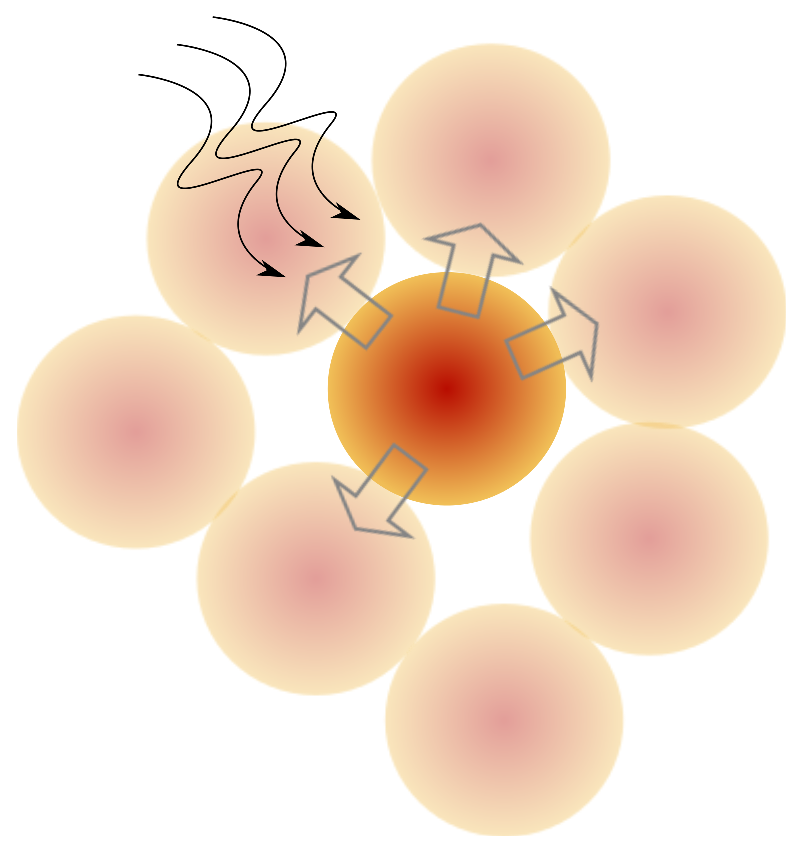
\includegraphics[width=0.75\textwidth]{chapters/figures/pebble-complete-heat-transfer}\label{fig:peb-comp-ht}
\end{figure}



\begin{enumerate}
\item Conduction through the contact area between contacting particles.
\item Conduction through the stagnant fluid between near, non-contacting particles.
\item Conduction through the stagnant fluid between contacting particles.
\item Conduction through the interstitial fluid. 
\item Advection of the fluid to contacting- and downstream particles.
\item Radiation between the surfaces of contacting particles.
\item Radiation between particles of adjacent voids.
\item Heat generation internally in the particle.
\end{enumerate}

The first mode of transfer will be addressed in \S\ref{sec:ht-pebble-conduction} where we will go through the development of a form of heat conductance between contacting, elastic spheres. Ideally, modes 2-5 would each receive separate treatment but we will wrap up all of their influences with heat transfer coefficients that are functions of local packing fraction to account for both the fluid and the neighboring particles; this is done in \S\ref{sec:particle-convection}. For the present study, we will entirely neglect the modes 6, and 7 because of their added complexity. Finally, the last mode of heat transfer is trivially accounted for with a heat source term,

\begin{equation}\label{eq:nuclear-heating-term}
	Q_g = q'''V
\end{equation}

where $q'''$ is a known volumetric heating rate and $V$ is the volume of our particle. In practice, we will know a volumetric heating rate from the location and geometry of the solid breeder volume. The volume of the sphere is $V = \frac{4}{3}\pi R^3$.

In the following sections we will expand upon the details of the modes of heat transfer considered for our packed beds. They forms of equations used will be written in a way to be implemented directly into the DEM computational framework, to be discussed later in \S\ref{modeling-DEM}.

% The transient energy balance for an irradiated pebble, shown in Fig.~\ref{fig:peb-comp-ht}, in a packed bed with flowing interstitial gas is given by Eq.~\ref{eq:single-pebble-energy},

% \begin{equation}\label{eq:single-pebble-energy}
% 	\rho V C \frac{\mathrm{d}T}{\mathrm{d}t} = \dot{Q}_g + \dot{Q}_\text{conduction} + \dot{Q}_\text{convection} + \dot{Q}_\text{radiation}
% \end{equation}



%%%%%%%%%%%%%%%%%%%%%%%%%%%%%%%%%%%%%%%%%%
\subsection{Inter-particle heat conduction}\label{sec:ht-pebble-conduction}

When two particles come into contact, energy is transmitted through their region of contact. For this discussion, we assume the particles are spherical, elastic, in vacuum, and we neglect radiation transfer between them. If the two particles are at temperatures $T_i$ and $T_j$ we can quantify the amount of energy transferred between them with a commonly used practice of a contact conductance, $H_c$:
\begin{equation}\label{eq:pebble-conduction-heat-transfer}
	Q_{ij} = H_{c}(T_i - T_j)
\end{equation}

The subscripts are omitted for clarity, but obviously there is a unique $H_c$ per pair of contacting particles. We note that the heat conductance, unlike standard heat transfer coefficients, has units of \si{W/K}.

Batchelor and O'Brien\cite{Batchelor1977} developed a formulation of similar form and then made the brilliant observation that the temperature fields in the near-region of contacting spheres are analogous to the velocity potential of an incompressible, irrotational fluid passing from from one reservoir to another through a circular hole in a planar wall separating the two reservoirs. With the analogy, they could make use of the fluid flow solution to write the total flux across the circle of contact just as Eq.~\ref{eq:pebble-conduction-heat-transfer} with the heat conductance as

\begin{equation}\label{eq:batchelor-pebble-conductance}
	H_c = 2k_ra
\end{equation}

where $k_r$ is the conductivity of the contacting solids and $a$ is the radius of contact. In \cref{sec:hertz-theory}, with Hertz theory we found the contact radius in terms of the contact pressure. Here, we give the radius in terms of the compression force acting on the bodies,

\begin{equation}
	a =  \left(\frac{3}{4}\frac{R^*}{E^*}\right)^{1/3}F_n^{1/3}	
\end{equation}

as before, $\frac{1}{E^*} = \frac{1-\nu_1^2}{E_1} + \frac{1-\nu_2^2}{E_2}$ and $\frac{1}{R^*} = \frac{1}{R_1} + \frac{1}{R_2}$. 

In the development of Eq.~\ref{eq:batchelor-pebble-conductance}, Batchelor and O'Brien had assumed the two contacting spheres to be of equal conductivity, $k_r$. Cheng, et al.\cite{Cheng19994199} proposed a slightly modified conductance which allows for contacting materials of different thermal conductivity. They have,

\begin{equation}\label{eq:cheng-modification-batchelor}
	H_c = 2k^*a = 2k^* \left(\frac{3}{4}\frac{R^*}{E^*}\right)^{1/3}F_n^{1/3}
\end{equation}

where $\frac{1}{k^*} = \frac{1}{k_i} + \frac{1}{k_j}$. As well as being a more general, flexible formulation, the models analyzed by Cheng, et al.\cite{Cheng19994199} are in good agreement with experiments. In the DEM numerical structure, we use the form given by Eq.~\ref{eq:cheng-modification-batchelor}.

Furthermore, Batchelor and O'Brien developed Eq.~\ref{eq:batchelor-pebble-conductance} with the assumption of two contacting particles in vacuum but, once developed, showed\cite{Batchelor1977} that this form is still valid when immersed in a fluid providing that the thermal conductivity ratio of solid and fluid is well above unity. The condition is expressed as,

\begin{equation}\label{eq:conductance-validity-fluid}
	\frac{ k_r }{ k_f } \frac{a}{R^*} \gg 1
\end{equation}

The term $\frac{a}{R^*}$, from \cref{sec:hertz-theory}, is necessarily much less than 1 for Hertz theory to be applicable. Thus for fluid in vacuum, the condition is identically satisfied but we must consider inaccuracies if we introduce an interstitial fluid with low conductivity ratios; for lithium ceramics in helium, the ratio is approximately $\frac{k_r}{k_f} \approx 10$.

As we step back from the contact of a single pair of particles and consider a particle in an ensemble with many contacts, we must again consider the validity of applying Eq.~\ref{eq:cheng-modification-batchelor} at each contact. Vargas and McCarthy\cite{Vargas2002a}, proposed introducing a conduction Biot number to relate resistance to heat transfer internal to the particle with the resistance between particles. We use the following form

\begin{equation}
	\Bi_c = \frac{H_c}{k^* d_p} = 2\frac{a}{d_p}
\end{equation}

Then if $\Bi_c \ll 1$, the individual energy transferred between each point of contact can be decoupled. The Biot number criteria is already satisfied for Hertz theory to be valid; having assumed that $\frac{a}{d_p} \ll 1$. Therefore the total heat transferred out of a single particle with $Z$ contacts is the summed contribution of individual contacts, 

\begin{equation}
	Q_i = \sum_j^Z Q_{ij}
\end{equation}

The contact conductance we use, Eq.~\ref{eq:cheng-modification-batchelor}, which is built upon the solution of Batchelor and O'Brien\cite{Batchelor1977}, has been implemented by others in a variety of studies\cite{Vargas2001, Chaudhuri2006, Zhou2009,Cheng19994199}. However, in many other fields, the researchers are interested in such things as the parallel conduction through a stagnant interstitial gas\cite{Bu2013} or the temporary conduction during impact of fluidized beds\cite{Zhu2008,Zhang2011,Wu2011,Li2000}. In such cases, the formula for conductance can be quite different but are not appropriate for the physics of our packed beds.

% Nevertheless, for the packed beds of ceramic spheres for which we are working towards modeling, the heat conductance of Eq.~\ref{eq:cheng-modification-batchelor} is an appropriate and valid form. The interstitial gas, be it stagnant or moving, will be incorporated the influence of an interstitial gas, it will be done in such a way as to leave the DEM heat transfer intact and only add an energy source term to stand in for the interaction with the fluid. The details will be discussed in \cref{sec:cfdem-heat-transfer}, but for now we conclude with a solid conduction theory that will be implemented in the discrete element method computations.
\section{Nusselt number for spheres in packed beds}\label{sec:particle-convection}
\subsection{Convection by interstitial gas}

Engineers have paid considerable attention to the calculation of convective heat transfer in packed beds. Correlations for determining the Nusselt number of a sphere in dilute and dense packings over a range of Reynolds and Prandtl number are available. We will cover the detail of many of these correlations in \S\ref{sec:}. The methods all come down to calculating Nusselt number to find the heat transfer coefficient and then computing the rate of heat transfer from convection as

\begin{equation}
	\dot{Q}_\text{convection} = -hA(T_s-T_f)
\end{equation}

where $T_s$ is the temperature of the solid with surface area, $A$, and $T_f$ is the local bulk temperature of the passing fluid. The negative sign is to maintain convention that energy transfer into the solid is positive.

\section{Jeffreson correction to lumped capacitance method}\label{sec:ht-jeffreson-correction}
In \S\ref{sec:particle-convection}, we discuss correlations for heat transfer coefficients of spheres in a packed bed. Then those correlations are utilized with CFD-DEM computational routines in \S\ref{eq:cfdem-dem-energy}. When implemented in the DEM-based modeling, we make the lumped capacitance assumption for each particle in the ensemble. The assumption eases the computational efforts of solving for the temperature distribution inside each particle; each particle is treated as isothermal. The accuracy of the lumped capacitance method is described by the Biot number,

\begin{equation}
     \Bi = \frac{hd_p}{k_r}
\end{equation} 

and for $\Bi \ll 1$ the lumped capacitance method accurately models the behavior of a solid interacting with a fluid. For $\Bi \approx 0.1$, the error from the lumped capacitance method is only about 5\%. In solid breeder volumes, the particles are generally small, solid conductivity low, and heat transfer coefficient generally also low. This leads to small-to-moderate Biot numbers expected in the packed bed. In this section we will analyze the accuracy of the lumped capacitance and introduce a correction method to account for inaccuracies of the method at moderate Biot numbers.

We simplify the case of a packed bed and only consider a single sphere with volumetric heat generation submerged in and thermally interacting with a fluid. The sphere will be of radius $R=d_p/2$, as shown in Fig.~\ref{fig:ParticleControlVolume}. The sphere will initially be at a uniform temperature of $T_i$. The fluid temperature will remain constant at $T_f$

\begin{figure}[ht]
	\centering
		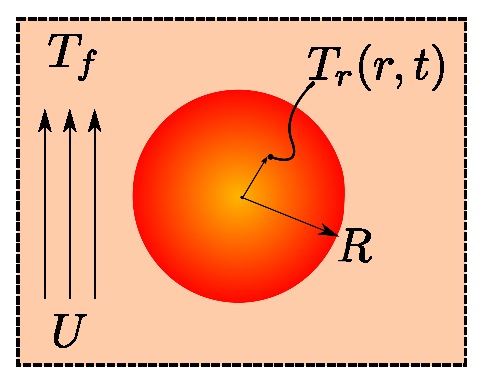
\includegraphics[width=2in]{chapters/figures/ParticleControlVolume}
	\caption[Control volume of single spherical particle in a packed bed]{CONTROL VOLUME OF A SINGLE SPHERICAL PARTICLE IN A PACKED BED}
	\label{fig:ParticleControlVolume}
\end{figure}


%~~~~~~~~~~~~~~~~~~~~~~~~~~~~~~~~~~~~~~~~~~~~~~~~~~~~~~~
\subsection{Lumped capacitance solution for sphere}\label{sec:lumped-capacitance}
We will solve for a single sphere interacting with a passing fluid, as shown in Fig.~\ref{fig:ParticleControlVolume}. We make the lumped capacitance assumption for this sphere. The solid is initially at temperature $T_0$, with constant volumetric heat generation, cooling in a fluid with constant heat transfer coefficient. The fluid will remain constant at $T_f$.

The time response of the sphere's temperature is dictated by the balance of energy to/away from the solid,  

\begin{equation}\label{eq:lc-energy-balance}
	\rho_rC_rV\frac{dT}{dt} = -hA(T-T_f) + gV
\end{equation}

Eq.~\ref{eq:lc-energy-balance} is solved in dimensionless form with the following nondimensional parameters of temperature and time,

\begin{subequations}
\begin{align}
    \theta &= \frac{T(t) - T_f}{T_0 - T_f}\\
    \tau & = \frac{t}{R^2/\alpha}
\end{align}
\end{subequations}

where $\alpha$ is the thermal diffusivity of the sphere, $T_0$ is the initial isothermal temperature of the sphere, and $T_f$ is the constant fluid temperature. The resulting temperature distribution is,

\begin{equation}
\label{eq:theta-lc}
	\theta_{LC}=\left(1-\frac{G}{3\Bi}\right)\exp(-3\Bi \tau) + \frac{G}{3\Bi}
\end{equation}

where we define a dimensionless heat generation,

\begin{equation}\label{eq:nondimensional-heat-generation}
	G = \frac{gR^2}{k(T_0 - T_f)}
\end{equation}

The energy of the sphere, relative to the fluid, in nondimensional terms is 

\begin{equation}
    E^*(\tau)=\frac{E(\tau)}{E_0}
\end{equation}

where $E_0$ is the initial energy of the sphere,

\begin{equation}
    E_0=\rho_rC_rV(T_0-T_f)
\end{equation}

Thus for a sphere with the lumped capacitance model, in nondimensional form, is simply

\begin{equation}\label{eq:lc-energy-profile}
	E^*_{LC}(\tau) = \theta_{LC}(\tau)
\end{equation}

The nondimensional energy profile of Eq.~\ref{eq:lc-energy-profile} is plotted over the nondimensional time of $\tau \in [0,1/\Bi]$ in Fig.~\ref{fig:LC-sphere-in-fluid}. 

\begin{figure}[ht]
	\centering
		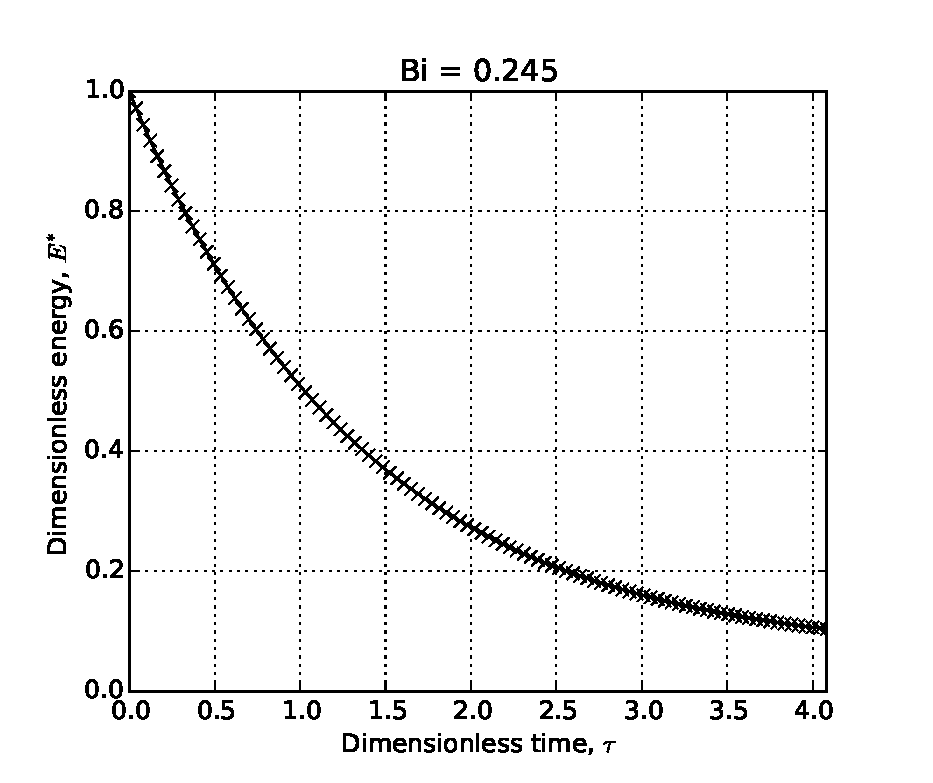
\includegraphics[width=0.75\textwidth]{chapters/figures/LC-sphere-in-fluid}
	\caption[Lumped Capacitance energy profile]{Lumped capacitance model: Sphere energy profile decaying from an initial value to a time of $1/\Bi$}
	\label{fig:LC-sphere-in-fluid}
\end{figure}

Reviewing Eq.~\ref{eq:theta-lc} we see that the speed of decay is dictated by the term in the exponential, $3\Bi$. Meanwhile, the steady-state value being approached is given by $\frac{G}{3\Bi} = \frac{gR}{h(T_0 - T_f)}$. It is important for this discussion to point out that because both the nondimensional heat generation and Biot number terms contain the solid conductivity, the steady-state value of the lumped capacitance model will not change for varying solid conductivity even if it leads to different Biot numbers. We will return to this point in the next section when we compare the lumped capacitance model to the exact solution when internal conduction of the solid is considered.
%~~~~~~~~~~~~~~~~~~~~~~~~~~~~~~~~~~~~~~~~~~~~~~~~~~~~~~~



%~~~~~~~~~~~~~~~~~~~~~~~~~~~~~~~~~~~~~~~~~~~~~~~~~~~~~~~
\subsection{Exact solution for sphere}\label{sec:analytic-sphere}

We again analyze the sphere of Fig.~\ref{fig:ParticleControlVolume} but now will account for internal temperature gradients inside the sphere. The details of the analytic solution for a sphere with heat generation interacting with a fluid is given in Appendix~\ref{sec:analytic-sphere-details}. We again solve in terms of the nondimensional temperature and time introduced in \S\ref{sec:lumped-capacitance} as well as a nondimensional radius,

\begin{align*}
    \theta &= \frac{\mathbb{T}}{\mathbb{T}_0}\\
    \rho & = \frac{r}{R}\\
    \tau & = \frac{t}{R^2/\alpha}
\end{align*}

The energy conservation equation for the sphere with internal temperature gradient, in nondimensional form $\theta_{TG}$, is

\begin{equation}
    \frac{1}{\rho}\frac{\partial^2}{\partial \rho^2}(\rho\theta_{TG}) + G = \frac{\partial\theta_{TG}}{\partial \tau}
\end{equation}

With the initial condition and boundary conditions outlined in Appendix~\ref{sec:analytic-sphere-details}, the nondimensional temperature distribution inside the sphere is 

\begin{equation}\label{eq:analytic-temperature-distribution}
    \theta_{TG}(\rho,\tau) = \left(\frac{G}{6} + \frac{G}{3\Bi}-\rho^2\right)  +   \sum_{n=1}^\infty \exp(-\zeta^2 \tau) \frac{\sin(\zeta_n \rho)}{\rho} \frac{Z(\zeta_n)}{N(\zeta_n)}  
\end{equation}

where $\zeta_n$ are the eigenvalues of the equation and the functions of $\zeta_n$ ($Z$,$N$,$C$) are given in Appendix~\ref{sec:analytic-sphere}. 

The accompanying nondimensional energy of the sphere is integrated to,

\begin{equation}
\label{eq:analytic-energy-profile}
    E^*_{TG}(\tau)=\left(\frac{G}{15}+\frac{G}{3\Bi}\right)+3\sum_{n=1}^\infty \exp(-\zeta^2 \tau) \frac{Z(\zeta_n)}{N(\zeta_n)} C_n(\zeta_n)
\end{equation}

We now compare the exact solution from Eq.~\ref{eq:analytic-energy-profile} to the solution of energy given by the lumped capacitance model of Eq.~\ref{eq:lc-energy-profile}. The two profiles are given in Fig.~\ref{fig:LC-analytic-sphere-in-fluid}. 

\begin{figure}[ht]
	\centering
		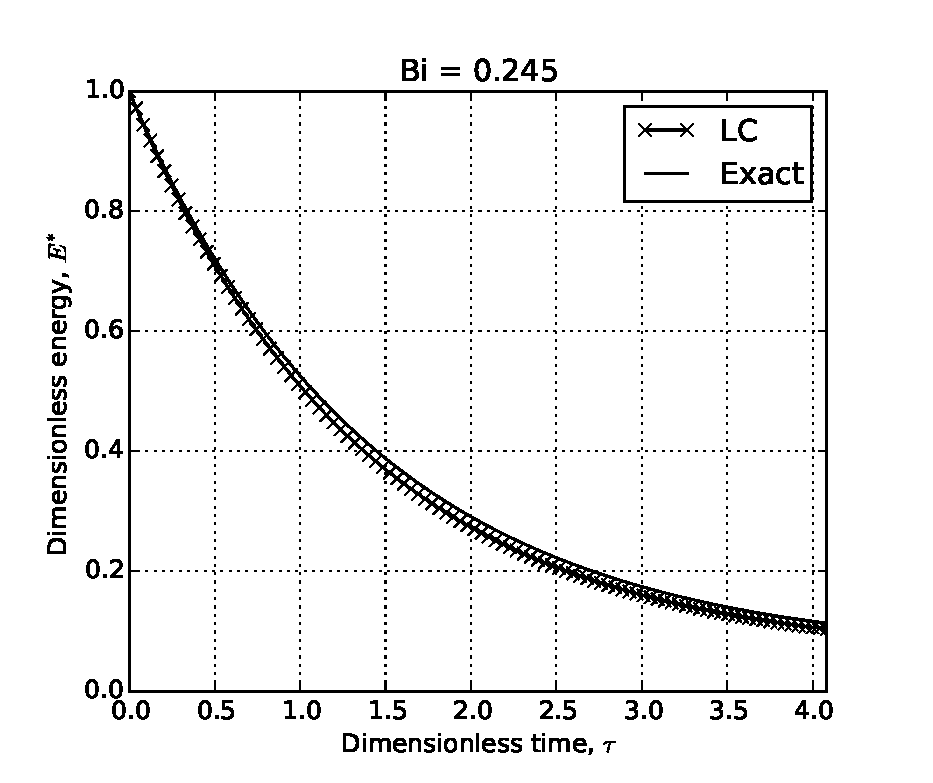
\includegraphics[width=0.75\textwidth]{chapters/figures/LC-analytic-sphere-in-fluid}
	\caption[Analytic temperature profile for $\Bi < 1$]{Analytic and lumped capacitance models: Sphere energy profile decaying from an initial value to a time of $1/\Bi$}
	\label{fig:LC-analytic-sphere-in-fluid}
\end{figure}

For the value of Biot number here, $\Bi < 0.5$, the profile of the analytic solution of the sphere is well-captured by the lumped capacitance model. The maximum relative error over the time span, as defined by

\begin{equation}\label{eq:error}
	\text{error} = \frac{\big|E^*_{TG}(\tau) - E^*_{LC}(\tau) \big|}{E^*_{TG}(\tau)}
\end{equation}

is always less than 10\%. 

We consider now the same size sphere but with the Biot number increased by an order by: a) a conductivity of $k = k_r/10$ and b) a heat transfer coefficient of $h = 10h_f$. The two physical changes to the system result in the same Biot number but as we can see in Fig.~\ref{fig:LC-analytic-sphere-in-fluid-Bi-2}, there are drastic changes in the results. 

\begin{figure}
        \centering
        \begin{subfigure}[b]{0.5\textwidth}
                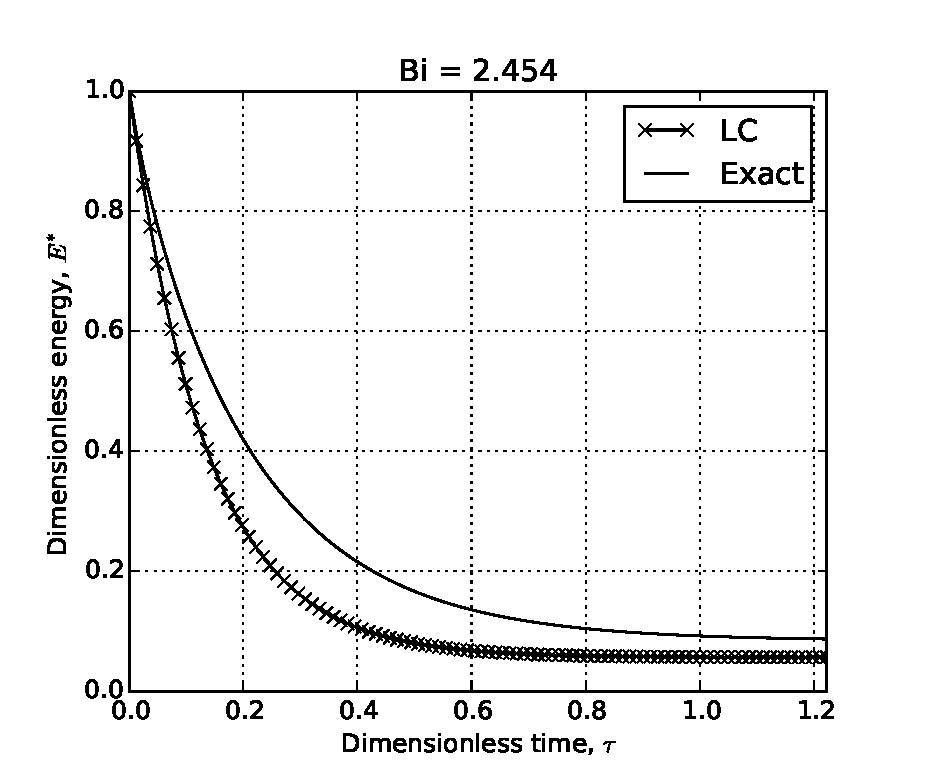
\includegraphics[width=\textwidth]{chapters/figures/LC-analytic-sphere-in-fluid-Bi-2a}
                \caption{The Biot number increased from a decrease in the solid conductivity.}
				\label{fig:LC-analytic-sphere-in-fluid-Bi-2a}
        \end{subfigure}%
        
          %add desired spacing between images, e. g. ~, \quad, \qquad, \hfill etc.
          %(or a blank line to force the subfigure onto a new line)
        \begin{subfigure}[b]{0.5\textwidth}
                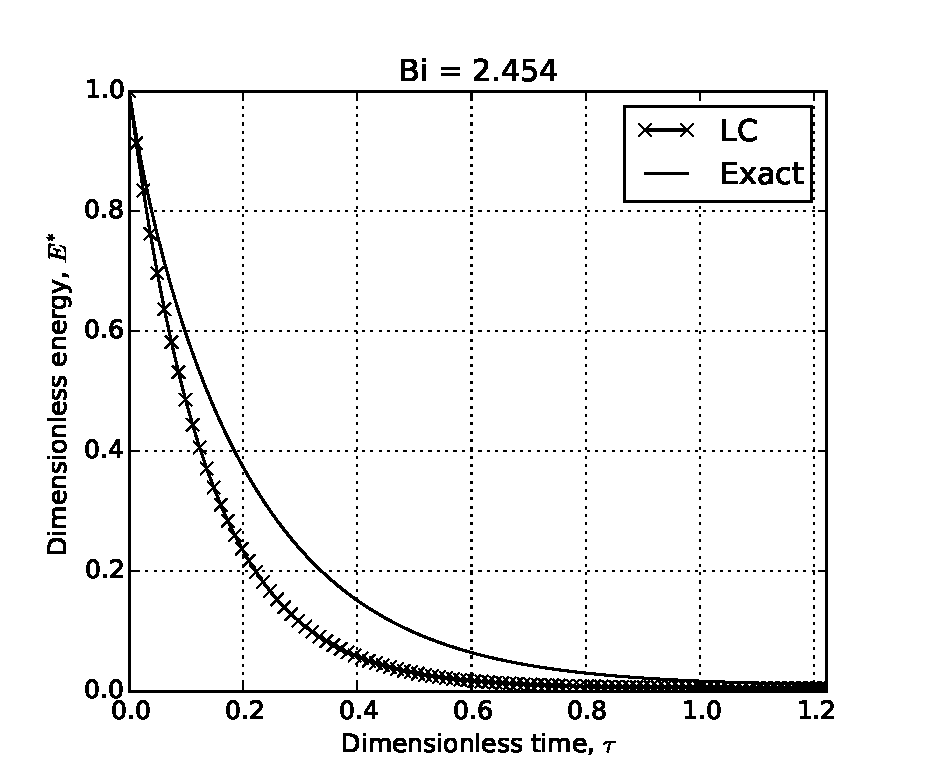
\includegraphics[width=\textwidth]{chapters/figures/LC-analytic-sphere-in-fluid-Bi-2b}
                \caption{The Biot number increased from  an increase in the heat transfer coefficient.}
				\label{fig:LC-analytic-sphere-in-fluid-Bi-2b}
        \end{subfigure}
        \caption[Analytic temperature profile for moderate Biot number]{Analytic and lumped capacitance models: Sphere energy profile decaying from an initial value to a time of $3/\Bi$. The same Biot number produces different results for the exact solution of a sphere with heat generation.}\label{fig:LC-analytic-sphere-in-fluid-Bi-2}
\end{figure}

Seen in Fig.~\ref{fig:LC-analytic-sphere-in-fluid-Bi-2a}, the lumped capacitance solution both over-predicts the speed at which the sphere reaches a thermal steady-state as well as the value of the steady-state. Comparatively, in Fig.~\ref{fig:LC-analytic-sphere-in-fluid-Bi-2b}, for the same Biot number the lumped capacitance solution again over-predicts the speed to thermal steady-state by the same rate but is relatively accurate for the steady-state value itself. 

To first address the source of error on the steady-state value, we view the steady-state terms of the two solutions. From Eq.~\ref{eq:analytic-energy-profile}, we write the steady-state term of the exact solution as 

\begin{equation}
	E^*_{TG,ss}=\frac{G}{15}+\frac{G}{3\Bi}
\end{equation}

Comparatively, we write the steady-state term of the lumped capacitance solution from \S\ref{sec:lumped-capacitance} as,

\begin{equation}
	E^*_{LG,ss} = \frac{G}{3\Bi}
\end{equation}

We clearly see that the two steady-state values differ by the contribution of $\frac{G}{15}$ on the exact solution. This term does not appear in the lumped capacitance solution because it does not account for the temperature difference through the sphere. The nondimensional heat generation term is given in Eq.~\ref{eq:nondimensional-heat-generation}; it is importantly a function of thermal conductivity but not the heat transfer coefficient. This explains the difference between steady-state values in Fig.~\ref{fig:LC-analytic-sphere-in-fluid-Bi-2} when we modified the two parameters.

To address the inaccuracies in the time-dependent response of the lumped capacitance method with large Biot number, we will make use of the so-called Jeffreson Correction described by Van Lew\cite{VanLew2010} and Xu et al.\cite{Xu2012}. In their work, they considered a heated heat transfer fluid interacting with a low conductivity thermal storage material. The solar thermal storage systems they analyzed often had moderate-to-large Biot numbers but they could continue to apply the lumped capacitance model by applying the Jeffreson Correction\cite{jeffreson409}. The details of the Jeffreson correction as applied to a system with volumetric heat generation will be discussed next.
%~~~~~~~~~~~~~~~~~~~~~~~~~~~~~~~~~~~~~~~~~~~~~~~~~~~~~~~





%~~~~~~~~~~~~~~~~~~~~~~~~~~~~~~~~~~~~~~~~~~~~~~~~~~~~~~~
\subsection{Jeffreson correction for sphere}
In Fig.~\ref{fig:LC-analytic-sphere-in-fluid-Bi-2}, the lumped capacitance model predicted a much faster decay to steady-state than the exact solution. Jeffreson summarized a correction to the lumped capacitance model via a reduction in the heat transfer coefficient as a function of the Biot number. The smaller heat transfer coefficient effectively slowed the decay to steady-state as predicted by the lumped capacitance method.
The correlation to correct the heat transfer coefficient due to solids with large Biot number is given by Jeffreson\cite{jeffreson409}. The Jeffreson correction for a sphere is,

\begin{equation}
	h_{p}=\frac{h}{1+\Bi/5}
\end{equation}

where $h_p$ is the modified heat transfer coefficient of the particle with an internal temperature gradient.  An increase in the Biot Number (or increase of thermal gradient inside the solid) results in a decrease in the heat transfer coefficient~$h_p$. A modified Biot number can then also be written as

\begin{equation}\label{eq:jeffreson-correction-bip}
	\Bi_p = \frac{h_p d}{k_r} = \frac{\Bi}{1+\Bi/5}
\end{equation}

Applying the Jeffreson Correction to Eq.~\ref{eq:theta-lc},

\begin{equation}
\label{eq:theta-jc-bip}
	\theta_{JC}=\left(1-\frac{G}{3\Bi_p}\right)\exp\left(-3\Bi_p \tau\right) + \frac{G}{3\Bi_p}
\end{equation}

and thereby Eq.~\ref{eq:lc-energy-profile} gives

\begin{equation}\label{eq:jc-energy-profile}
	E^*_{JC}(\tau) = \theta_{JC}(\tau)
\end{equation}

We then plot the energy profiles from the lumped capacitance model (LC), the Jeffreson correction (JC), and the exact solution together in Fig.~\ref{fig:LC-JC-analytic-sphere-in-fluid-Bi-2}

\begin{figure}
        \centering
        \begin{subfigure}[b]{0.5\textwidth}
                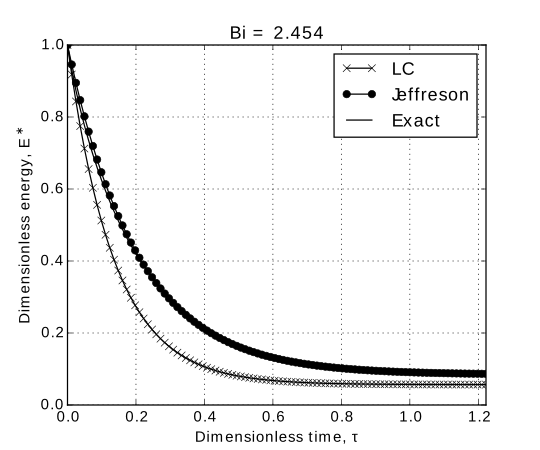
\includegraphics[width=\textwidth]{chapters/figures/LC-JC-analytic-sphere-in-fluid-Bi-2a}
                \caption{The Biot number increased from a decrease in the solid conductivity.}
				\label{fig:LC-JC-analytic-sphere-in-fluid-Bi-2a}
        \end{subfigure}%
        
          %add desired spacing between images, e. g. ~, \quad, \qquad, \hfill etc.
          %(or a blank line to force the subfigure onto a new line)
        \begin{subfigure}[b]{0.5\textwidth}
                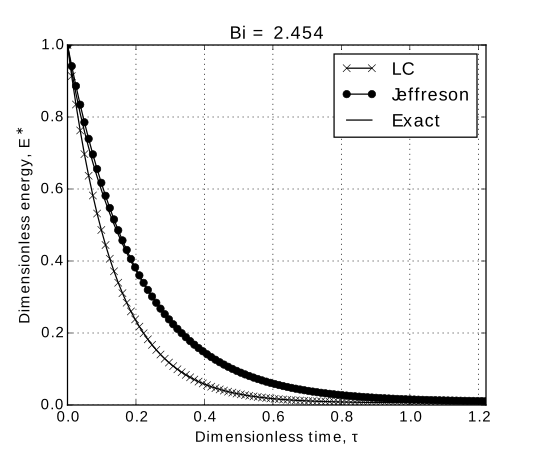
\includegraphics[width=\textwidth]{chapters/figures/LC-JC-analytic-sphere-in-fluid-Bi-2b}
                \caption{The Biot number increased from  an increase in the heat transfer coefficient.}
				\label{fig:LC-JC-analytic-sphere-in-fluid-Bi-2b}
        \end{subfigure}
        \caption[Jeffreson correction for moderate Biot number based on conductivity]{Analytic, lumped capacitance model, and LC model with Jeffreson correction: Jeffreson correction corrects for transient and steady-state errors of lumped capacitance.}\label{fig:LC-JC-analytic-sphere-in-fluid-Bi-2}
\end{figure}

The Jeffreson correction to the lumped capacitance method allows the simple model to capture the proper transient as well as steady-state values for this sphere with a moderately sized Biot number. To look more closely, we view the instantaneous error (see Eq.~\ref{eq:error}) in Fig.~\ref{fig:LC-JC-analytic-error-Bi-2}.

\begin{figure}
        \centering
        \begin{subfigure}[b]{0.5\textwidth}
                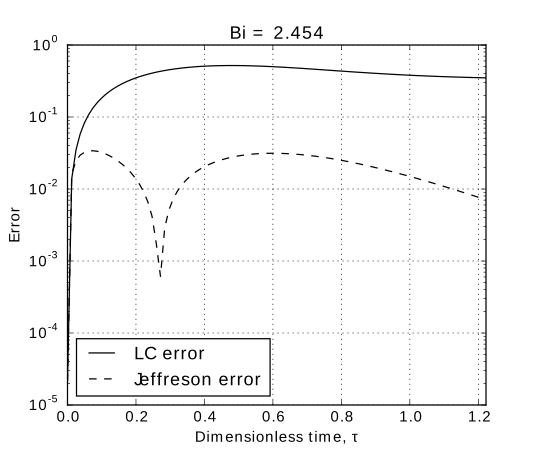
\includegraphics[width=\textwidth]{chapters/figures/LC-JC-analytic-error-Bi-2a}
                \caption{The Biot number increased from a decrease in the solid conductivity.}
				\label{fig:LC-JC-analytic-error-Bi-2a}
        \end{subfigure}%
        
          %add desired spacing between images, e. g. ~, \quad, \qquad, \hfill etc.
          %(or a blank line to force the subfigure onto a new line)
        \begin{subfigure}[b]{0.5\textwidth}
                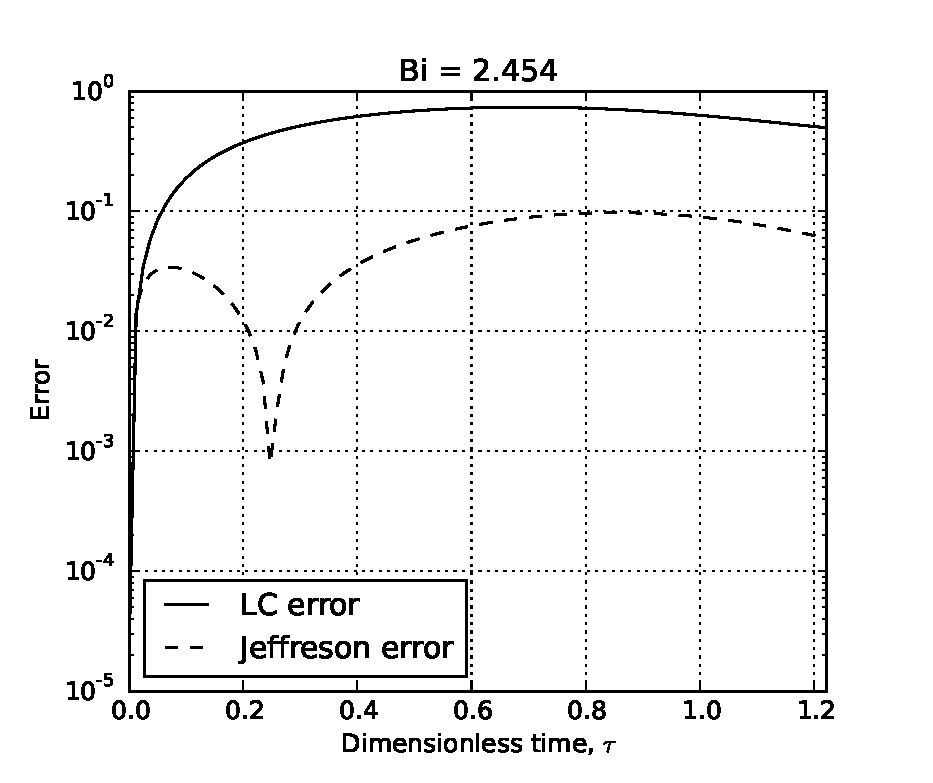
\includegraphics[width=\textwidth]{chapters/figures/LC-JC-analytic-error-Bi-2b}
                \caption{The Biot number increased from  an increase in the heat transfer coefficient.}
				\label{fig:LC-JC-analytic-error-Bi-2b}
        \end{subfigure}
        \caption[Error of lumped capacitance and Jeffreson correction for moderate Biot number]{Error of lumped capacitance and reduced error of the model with Jeffreson correction for moderate Biot number.}\label{fig:LC-JC-analytic-error-Bi-2}
\end{figure}

For the value of $\Bi > 1$ due to either low conductivity (Fig.~\ref{fig:LC-JC-analytic-error-Bi-2a}) or high heat transfer coefficient (Fig.~\ref{fig:LC-JC-analytic-error-Bi-2b}), the error in the Jeffreson correction is always under 10\%; often closer to only 1\%. This is in opposition to the standard lumped capacitance method which has 50-80\% error for both transient and steady-state values.

The lumped capacitance method allows researchers to simplify transient, conjugate heat transfer problems with an isothermal solid. In the discrete element method, the assumption of isothermal solid is innate in the framework of the method. With the implementation of the Jeffreson correction in the discrete element method, we have confidence in the fidelity of the heat transfer in for moderately sized Biot numbers. The Jeffreson correction will be implemented into the DEM computations via Eq.~\ref{eq:jeffreson-correction-bip}. 
%~~~~~~~~~~~~~~~~~~~~~~~~~~~~~~~~~~~~~~~~~~~~~~~~~~~~~~~
\subsection{Radiative transfer with neighboring particles}

The temperatures expected in the solid breeder are high enough that we can not a priori neglect radiation. The radiation exchange between contacting neighbors in a packed bed becomes extremely complex due to the local and semi-local nature of radiation. A standard approach to treat radiation exchange between surfaces is to consider the view factor between them. In a dense, randomly packed bed of spheres the computation of view factors between pebbles can be done via a method such as that proposed Feng and Han\cite{Feng2012}. Ideally, we could show this mode of heat transport is negligible compared to the others already discussed.

In ceramic breeder designs, the tritium breeding volume is rarely more than \si{2 cm} wide with pebbles that are, generally, \si{1 mm} in diameter. The maximum expected temperature in the breeding zone is about \si{1000 K}, roughly at the centerline of the \si{2 cm} width. The walls of the coolant must be held below the operable steel temperature of roughly \si{700 K}. This works out to a \si{300 K} differences spanning 10 pebble diameters. From this we can make a first-order approximation of \si{30 K} difference between neighboring pebbles. At the elevated temperatures, an estimate for the radiation exchange between two pebbles (allowing them to act as black bodies for this approximation) is

\begin{equation}
	\dot{Q}_\text{radiation} = \sigma A \left(T_\text{max}^4 - (T_\text{max}-30)^4\right) \approx 0.022\si{W}
\end{equation}
 
 which is the highest amount of radiation exchange we might expect between pebbles. Even though we will neglect this mode of heat transfer for now, after reviewing some of the packed bed heat transfer results we may find that this quantity of energy transfer is not negligible and future versions of the model would have to account for it.
%%%%%%%%%%%%%%%%%%%%%%%%%%%%%%%%%%%%%%%%%%
